\chapter{Dati}
\label{ch:data}

GroundOne apprende un'unica decisione, quindi i dati devono insegnare esattamente quella decisione e permettere di
misurarla in modo affidabile. Il capitolo definisce anzitutto la decisione e le sue etichette. Descrive poi i tre
dataset pubblici da cui le etichette provengono e il modo in cui vengono trasformati in training set, dev set e test
set. Le ultime sezioni mostrano come l'affidabilità dei test set sia stata verificata senza nuove annotazioni, che cosa
emerge da un'analisi esplorativa del dataset costruito e come sia stato escluso il leakage tra i dati di addestramento e
quelli di test.

% Source of truth for every number in this chapter: Project/data/processed/groundone/DATACARD.md and
% build_report.json (dataset), Project/experiments/eda/report/eda_report.md and stats/ (exploratory analysis).

\section{Task ed etichette}
\label{sec:data-task}

L'input è costituito da un documento recuperato e da una risposta, scritta da un modello linguistico e suddivisa in
frasi. Per ogni frase il modello stabilisce se, \emph{rispetto al documento}, essa è \emph{supportata},
\emph{contraddetta} o \emph{non menzionata}. Una frase è supportata quando il documento dice, o implica direttamente,
tutto ciò che essa afferma. È contraddetta quando una sua parte è in conflitto con il documento. È non menzionata quando
aggiunge informazioni che il documento non contiene, ma nemmeno contraddice. Quando una frase contiene sia una parte in
conflitto sia una parte non verificabile, viene etichettata come contraddetta, perché la contraddizione è l'errore più
grave. Conta soltanto il documento: un'affermazione vera nel mondo reale ma assente dal documento resta non menzionata.

Il numero di decisioni richieste da una risposta coincide con il numero delle sue frasi valutate, indicato con $K$.
Questa grandezza è centrale nella tesi. Un decision model legge documento e risposta una sola volta, quindi ogni decisione aggiuntiva gli costa poco, soltanto i token della frase; un giudice generativo, invece, deve produrre testo per ogni frase. Per questo il
confronto con i giudici generativi è condotto in funzione di $K$, e i dati devono comprendere risposte lunghe oltre che
brevi.

Per ogni frase il modello restituisce tre probabilità, e ogni altra grandezza è derivata da queste, invece di essere
appresa separatamente. Il punteggio binario di groundedness, usato per il confronto con i benchmark binari pubblicati, è
$P(\text{supported})$. Le segnalazioni dipendono invece dalla nozione di errore adottata. Secondo una policy
\emph{strict} è un errore tutto ciò che il documento non afferma, e una frase viene segnalata quando
$P(\text{supported})$ scende sotto una soglia $\tau$. Secondo una policy \emph{lenient} sono errori soltanto le
contraddizioni, e una frase viene segnalata solo quando è giudicata contraddetta. In questo modo l'utente sceglie la
nozione di errore e la soglia al momento dell'inferenza, senza riaddestrare il modello. La
Sezione~\ref{sec:method-calibration} riporta la regola esatta con cui il verificatore produce le etichette che
restituisce.

\section{Dataset di partenza}
\label{sec:data-sources}

Il dataset è costruito di proposito a partire dal minor numero possibile di fonti: una per l'addestramento e tre per il
test (Tabella~\ref{tab:data-sources}). Con meno fonti la definizione delle etichette e il formato del testo restano
unici, e si riducono i punti in cui la costruzione può introdurre errori.

\begin{table}[htbp]
\centering
\caption{I dataset di partenza: licenza, ruolo in GroundOne e tipo delle etichette originali.}
\label{tab:data-sources}
\small
\begin{tabularx}{\textwidth}{@{}>{\raggedright\arraybackslash}p{0.25\textwidth}>{\raggedright\arraybackslash}p{0.18\textwidth}>{\raggedright\arraybackslash}p{0.15\textwidth}>{\raggedright\arraybackslash}X@{}}
\toprule
Dataset & Licenza & Ruolo & Etichette \\
\midrule
RAGTruth~\cite{niu2024ragtruth} & MIT & Training set, dev set e test T1 & Span di caratteri delle risposte di LLM, annotati con quattro tipi di allucinazione (conflitto o informazione infondata, evidente o sottile). \\ \addlinespace
\mbox{LLM-AggreFact}~\cite{tang2024minicheck,llmaggrefact} & \mbox{CC BY-ND 4.0} & Solo test T2 & Un'etichetta binaria per ogni affermazione: supportata o non supportata. \\ \addlinespace
VitaminC~\cite{schuster2021vitaminc} & \mbox{CC BY-SA 3.0} & Solo test T3 & Tre classi per ogni affermazione: \emph{supports}, \emph{refutes} e \emph{not enough information}. \\
\bottomrule
\end{tabularx}
\end{table}

\paragraph{RAGTruth.} RAGTruth~\cite{niu2024ragtruth} contiene 17{,}790 risposte scritte da sei modelli linguistici
(GPT-3.5, GPT-4, Llama-2 7B, 13B e 70B, e Mistral-7B) in tre task di RAG, che si distinguono per il tipo di contesto.
Nel question answering il contesto è un insieme di passaggi recuperati per una domanda di MS~MARCO~\cite{nguyen2016msmarco}.
Nella summarization è un articolo di cronaca, tratto da CNN/DailyMail~\cite{hermann2015teaching,see2017pointer} o da
notizie recenti. Nella generazione data-to-text, in cui il modello descrive in prosa dati strutturati, il contesto è la
scheda di un'attività commerciale di Yelp in formato JSON~\cite{yelpdataset}. In ciascuna risposta, due annotatori
formati hanno individuato gli span di caratteri non supportati dal contesto\footnote{Uno \emph{span} è un tratto
contiguo di testo, individuato dalla posizione del suo primo e del suo ultimo carattere. Un'annotazione a livello di span
marca la porzione esatta della risposta che contiene l'errore, invece di giudicare la risposta nel suo insieme.}, con una
terza revisione nei casi di disaccordo. A ogni span hanno poi assegnato uno di quattro tipi: \emph{conflitto}, evidente o
sottile, e \emph{informazione infondata}, evidente o sottile. L'articolo riporta un accordo tra annotatori del 91.8\,\% a
livello di risposta e del 78.8\,\% a livello di span. RAGTruth è l'unico dataset pubblico che unisca risposte naturali di
più frasi, prodotte da modelli diversi, alla distinzione tra contenuto contraddetto e contenuto non supportato, ed è per
questo l'unica fonte di addestramento. Lo split ufficiale separa 450 fonti di test dalle restanti, destinate
all'addestramento.

\paragraph{LLM-AggreFact.} LLM-AggreFact~\cite{tang2024minicheck,llmaggrefact} aggrega undici dataset di fact checking
annotati manualmente, ciascuno composto da coppie (documento, affermazione). I dataset coprono tre ambiti: la
summarization (AggreFact-CNN e XSum~\cite{tang2023aggrefact}, TofuEval~\cite{tang2024tofueval}, con i due sottoinsiemi MediaS e MeetB), il question answering
basato su retrieval o con risposte in forma estesa (RAGTruth~\cite{niu2024ragtruth}, ClaimVerify~\cite{liu2023verifiability},
ExpertQA~\cite{malaviya2024expertqa}, LFQA~\cite{chen2024lfqa}) e il fact checking vero e proprio
(WiCE~\cite{kamoi2023wice}, REVEAL~\cite{jacovi2024reveal}, FactCheck-GPT~\cite{wang2024factcheckbench}). Il benchmark
ha una leaderboard pubblica, che rende i risultati confrontabili con quelli dei sistemi pubblicati. La sua licenza,
però, vieta di usare i dati per addestrare modelli~\cite{hf_llmaggrefact}. In questa tesi il dataset serve quindi
soltanto alla valutazione: nessun addestramento, calibrazione o selezione avviene su alcuno dei suoi split.

\paragraph{VitaminC.} VitaminC~\cite{schuster2021vitaminc,hf_vitaminc} è un dataset di verifica dei fatti costruito a
partire da revisioni di Wikipedia che cambiano un fatto. Per ogni revisione, annotatori formati hanno scritto
affermazioni supportate da una versione della frase e confutate dall'altra. Quando non era possibile formulare una
contraddizione, la coppia è stata etichettata come priva di informazioni sufficienti. Le due versioni dell'evidenza sono
quasi identiche, quindi per decidere il modello deve guardare al fatto preciso, e non alla sovrapposizione lessicale. Su
un campione ri-annotato di 2{,}000 coppie gli autori riportano un $\kappa$ di Fleiss pari a 0.71\footnote{Il $\kappa$
di Fleiss misura l'accordo tra più annotatori al netto dell'accordo che si otterrebbe per puro caso: vale 1 quando
l'accordo è perfetto e 0 quando non supera quello casuale.}. In questa tesi VitaminC colma una lacuna precisa. RAGTruth
non pubblica l'accordo tra annotatori sul \emph{tipo} di allucinazione, quindi da solo non può dimostrare che il modello
apprenda il confine tra contraddetta e non menzionata. VitaminC fornisce proprio questo confine, con etichette di
affidabilità nota e in un dominio diverso.

Diversi altri candidati sono stati esaminati e scartati. I corpora di NLI come ANLI~\cite{nie2020anli} hanno premesse
brevi, lontane dai contesti tipici della RAG, e la stessa distinzione a tre classi su testo fattuale è già coperta da
VitaminC. I dati di addestramento sintetici o soltanto binari, come quelli rilasciati con MiniCheck~\cite{tang2024minicheck},
non hanno etichette a tre classi. Infine, sono stati esclusi i dataset con etichette generate da un modello linguistico
e quelli che riutilizzano risposte di test di RAGTruth: in questo modo le etichette restano umane e i test set restano
indipendenti.

\section{Costruzione}
\label{sec:data-construction}

\paragraph{Segmentazione in frasi.} Le risposte contengono spesso elenchi e intestazioni, quindi vengono prima spezzate
in corrispondenza degli a capo. Ogni riga viene poi divisa in frasi con PySBD~\cite{sadvilkar2020pysbd}, un
segmentatore basato su regole che gestisce abbreviazioni e numeri decimali. I simboli di elenco iniziali, come ``3.'' o
``*'', vengono rimossi, perché riguardano l'impaginazione e non il contenuto. Lo stesso segmentatore è usato in
addestramento, in valutazione e in inferenza, così che il modello veda sempre frasi tagliate allo stesso modo. La Figura~\ref{fig:data-pipeline} riassume l'intero processo di costruzione, dalle fonti ai test set congelati.

\begin{figure}[htbp]
\centering
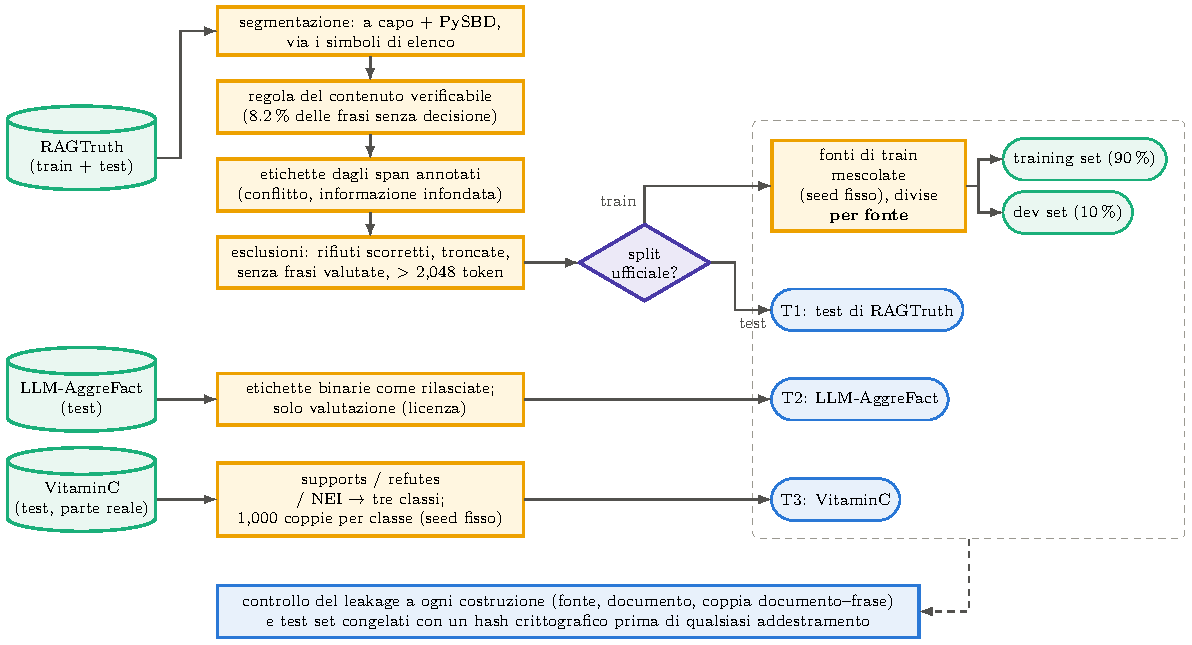
\includegraphics[width=\textwidth]{images/diagrams/data_pipeline_tikz.pdf}
\caption{Costruzione del dataset. Le risposte di RAGTruth sono segmentate, filtrate dalle frasi senza contenuto verificabile, etichettate a partire dagli span e ripulite dalle esclusioni; lo split ufficiale di test diventa T1, mentre le fonti di addestramento sono divise per fonte in training set e dev set. LLM-AggreFact e VitaminC forniscono soltanto test set (T2 e T3). Un controllo automatico del leakage accompagna ogni costruzione, e i test set sono congelati con un hash prima di qualsiasi addestramento.}
\label{fig:data-pipeline}
\end{figure}

\paragraph{Frasi senza contenuto verificabile.} Alcune frasi non affermano nulla sul documento: saluti, intestazioni
che introducono un elenco, righe che contengono soltanto una citazione, come ``(Passage 2)'', e formule di rifiuto.
Queste frasi restano nella risposta numerata come contesto, ma non costituiscono decisioni e non hanno etichetta. Una
breve regola le individua, e riguarda l'8.2\,\% di tutte le frasi di RAGTruth, in gran parte intestazioni di elenchi. La
regola considera soltanto la formattazione, cioè simboli di elenco, righe di sola citazione e formule conversazionali, e
non modifica mai un'etichetta. La sua copertura è stata verificata rispetto alla segmentazione indipendente di
LLM-AggreFact, descritta nella Sezione~\ref{sec:data-reliability}.

\paragraph{Etichette.} In RAGTruth l'etichetta di una frase valutata dipende dagli span con cui la frase si sovrappone.
La frase è contraddetta se si sovrappone a uno span di conflitto, non menzionata se si sovrappone soltanto a span di
informazione infondata, e supportata in tutti gli altri casi. Soltanto 27 dei 14{,}226 span annotati (0.19\,\%) non
toccano alcuna frase valutata, quindi la conversione non perde quasi nessuna annotazione. Per LLM-AggreFact, invece,
l'etichetta binaria è mantenuta così come rilasciata. Le etichette di VitaminC sono convertite direttamente:
\emph{supports} diventa supportata, \emph{refutes} contraddetta e \emph{not enough information} non menzionata. La Figura~\ref{fig:data-label-rule} riassume la regola applicata a RAGTruth.

\begin{figure}[htbp]
\centering
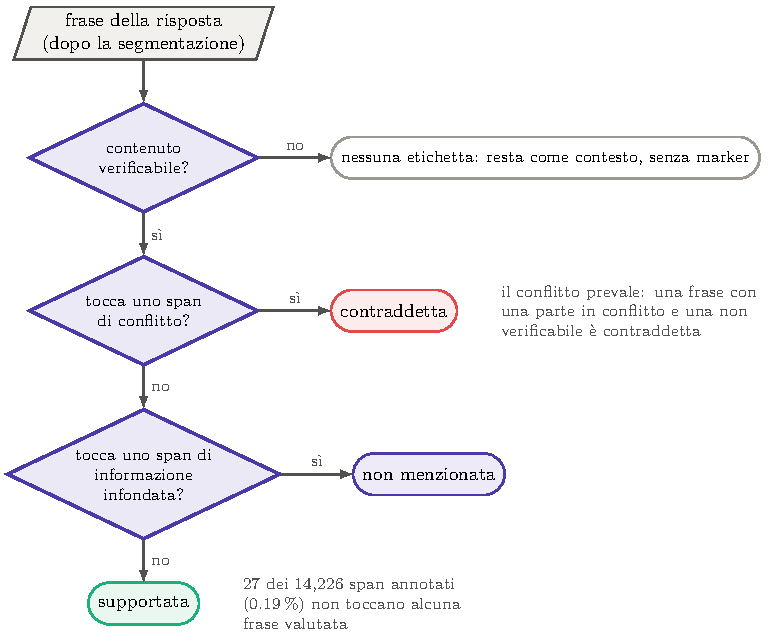
\includegraphics[width=0.85\textwidth]{images/diagrams/data_label_rule_tikz.pdf}
\caption{Regola con cui le annotazioni a livello di span di RAGTruth diventano etichette di frase. Le frasi senza contenuto verificabile restano nel prompt come contesto ma non sono decisioni; fra le altre, il conflitto prevale sull'informazione infondata.}
\label{fig:data-label-rule}
\end{figure}

\paragraph{Esclusioni e split.} Vengono rimosse tre categorie di risposte: quelle che RAGTruth segnala come rifiuti
scorretti o come troncate, quelle senza alcuna frase valutata e quelle in cui documento e risposta superano insieme i
2{,}048 token. Quest'ultimo limite di lunghezza è imposto dalla memoria del portatile da 16\,GB. Lo split di test
ufficiale di RAGTruth diventa il test set T1. Le fonti di addestramento, invece, vengono mescolate con un seed fisso e
divise in due parti: il 10\,\% forma il dev set e il resto il training set. Poiché la divisione avviene per fonte, le
risposte relative alla stessa fonte non compaiono mai in entrambi gli insiemi. Vengono inoltre rimosse sei risposte di
addestramento relative a un articolo di cronaca presente anche nel test set di LLM-AggreFact. Infine, la parte reale
(non sintetica) dello split di test di VitaminC è sbilanciata tra le classi, quindi T3 è formato campionando da essa,
con un seed fisso, 1{,}000 coppie per classe.

\section{Il dataset risultante}
\label{sec:data-result}

La Tabella~\ref{tab:data-splits} riassume i cinque file del dataset. Il training set contiene 13{,}203 risposte e
90{,}795 frasi etichettate. Ogni record corrisponde a una risposta e contiene un'etichetta per ciascuna frase: in questo
modo gli stessi dati possono alimentare modi diversi di leggere le $K$ decisioni di una risposta.

\begin{table}[htbp]
\centering
\caption{Il dataset GroundOne: numero di record e di decisioni per split e per classe. Una decisione è una frase
etichettata. T2 ha etichette binarie, quindi le frasi contraddette e non menzionate vi sono riunite nella classe non
supportata.}
\label{tab:data-splits}
\small
\begin{adjustbox}{max width=\textwidth}
\begin{tabular}{@{}llrrrrr@{}}
\toprule
Split & Fonte & Record & Decisioni & Supportate & Contraddette & Non menzionate \\
\midrule
Train & RAGTruth & 13{,}203 & 90{,}795 & 79{,}898 & 4{,}039 & 6{,}858 \\
Dev & RAGTruth & 1{,}468 & 9{,}996 & 8{,}827 & 410 & 759 \\
T1 & RAGTruth test & 2{,}647 & 17{,}284 & 15{,}745 & 584 & 955 \\
T2 & LLM-AggreFact test & 29{,}320 & 29{,}320 & 22{,}832 & \multicolumn{2}{c}{6{,}488 non supportate} \\
T3 & VitaminC test & 3{,}000 & 3{,}000 & 1{,}000 & 1{,}000 & 1{,}000 \\
\bottomrule
\end{tabular}
\end{adjustbox}
\end{table}

RAGTruth è fortemente sbilanciato: circa l'88\,\% delle frasi etichettate è supportato, e le contraddizioni sono appena
il 3--4\,\% (Figura~\ref{fig:data-balance}). Questa è la frequenza naturale degli errori nelle risposte dei modelli, e
viene preservata. Il test set riflette così ciò che un verificatore incontra nella pratica, mentre lo sbilanciamento
viene gestito in fase di addestramento. T3 compensa offrendo un test bilanciato fra le tre classi.

Le risposte contengono in media 6.9 frasi valutate nel training set e 6.5 in T1, con un massimo di 28
(Figura~\ref{fig:data-k}). Per analizzare i risultati in funzione della lunghezza, T1 è diviso in quattro fasce di $K$:
756 risposte con 1--4 frasi, 1{,}288 con 5--8, 497 con 9--13 e 106 con 14 o più. Quando una cella dei risultati contiene
meno di 30 frasi di una classe minoritaria, come accade per le frasi contraddette nel question answering, il valore
viene riportato ma segnalato come indicativo.

\begin{figure}[htbp]
\centering
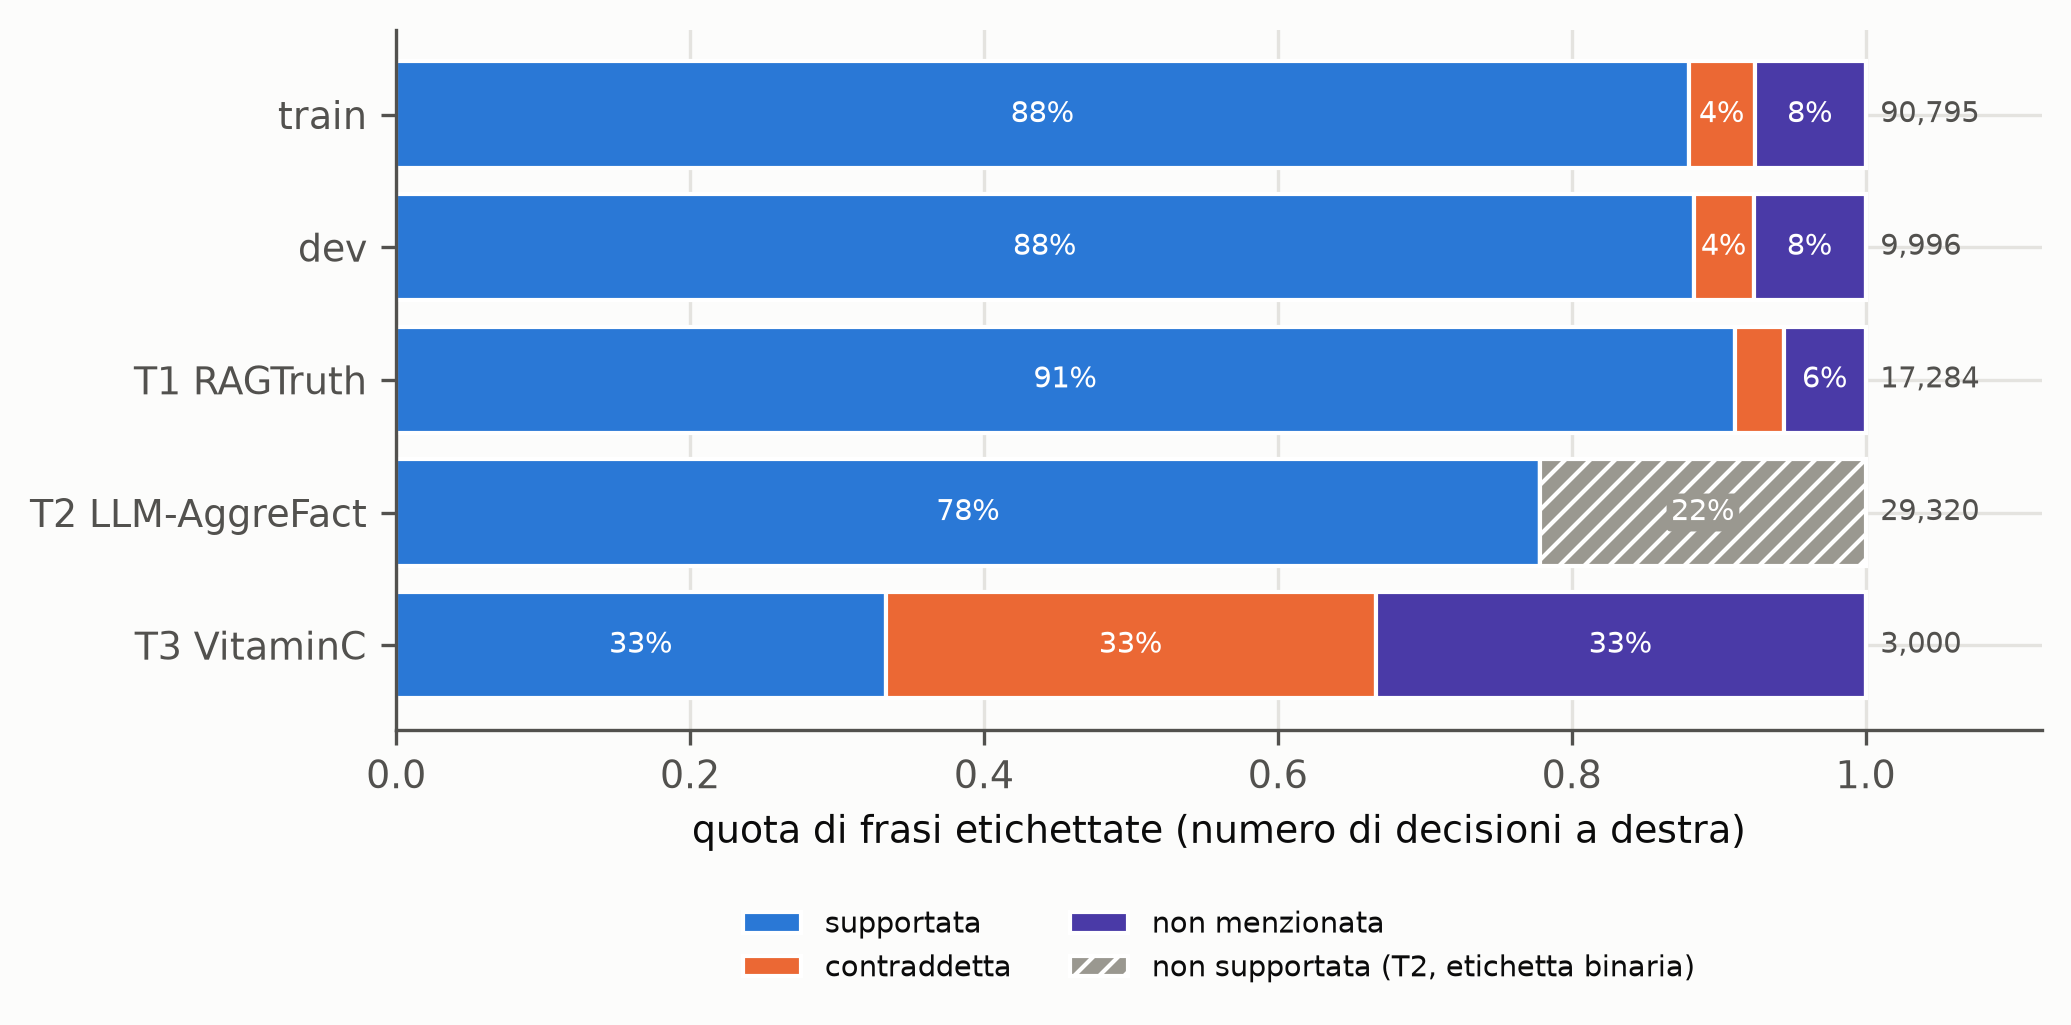
\includegraphics[width=0.9\textwidth]{images/dataset/class_balance_by_split.png}
\caption{Distribuzione delle classi fra le frasi etichettate di ciascuno split. Negli split di RAGTruth (train, dev e T1)
circa l'88--91\,\% delle frasi è supportato. T2 (LLM-AggreFact) ha etichette binarie, quindi le affermazioni
contraddette e non menzionate vi formano un'unica classe non supportata (tratteggio). T3 è campionato con 1{,}000
coppie per classe.}
\label{fig:data-balance}
\end{figure}

\begin{figure}[htbp]
\centering
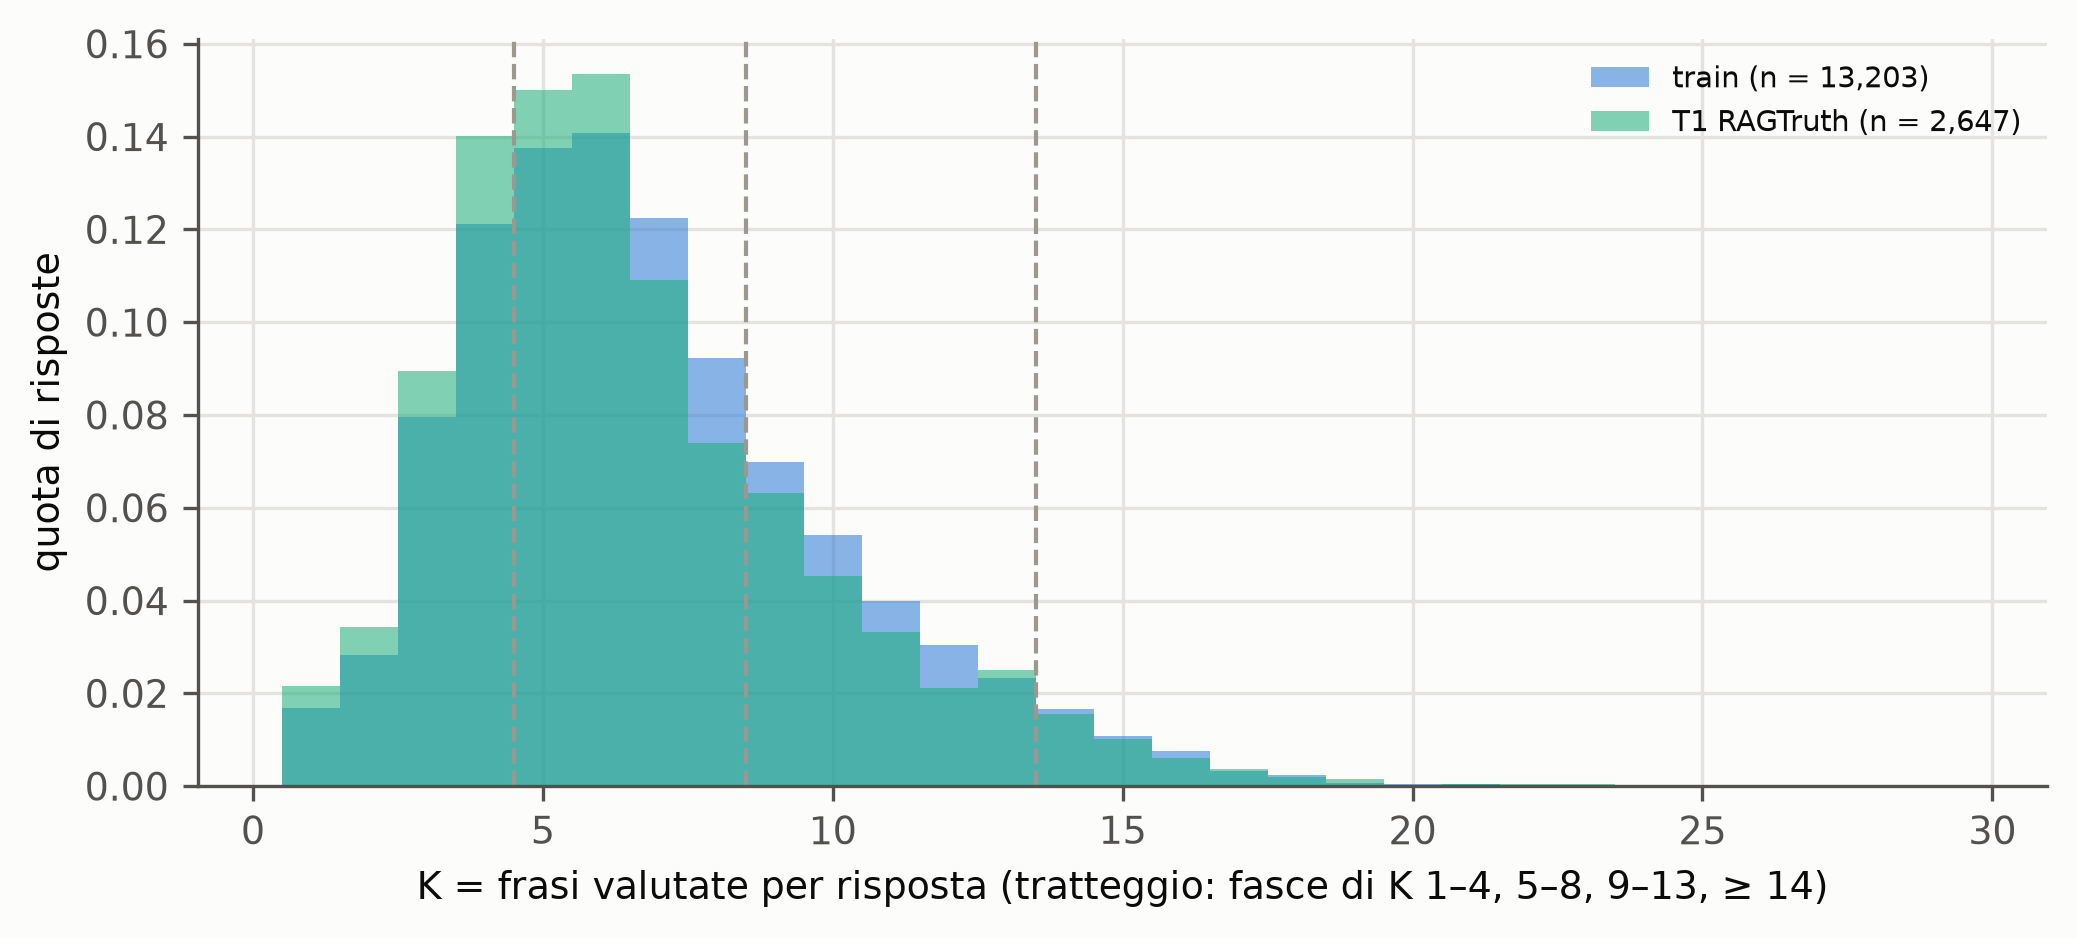
\includegraphics[width=0.9\textwidth]{images/dataset/K_distribution.png}
\caption{Distribuzione di $K$, il numero di frasi valutate per risposta, nel training set e in T1. Le linee
tratteggiate delimitano le fasce di $K$ usate per riportare i risultati.}
\label{fig:data-k}
\end{figure}

\section{Affidabilità dei test set}
\label{sec:data-reliability}

I test set sono stati verificati senza nuove annotazioni, ricorrendo a evidenze indipendenti dalla costruzione
descritta sopra (Tabella~\ref{tab:data-checks}). Tutte le etichette di test provengono dagli annotatori umani dei
dataset pubblicati. Le due scelte che potevano introdurre errori sono la segmentazione e la conversione dagli span alle
etichette di frase. Entrambe sono state confrontate con LLM-AggreFact, i cui autori hanno convertito in modo
indipendente le stesse risposte di test di RAGTruth in affermazioni a livello di frase. Il segmentatore di questa tesi
ritrova esattamente il 96.3\,\% delle loro affermazioni, e solo l'8.5\,\% delle frasi valutate è assente dal loro insieme. Si
tratta per lo più di frasi eliminate dal loro filtro delle affermazioni ``non meritevoli di verifica'', che non è
documentato. Sulle 15{,}492 frasi presenti in entrambi gli insiemi, le etichette binarie concordano nel 98.75\,\% dei
casi. Tutti i 193 disaccordi, inoltre, vanno nella stessa direzione: la regola basata sugli span marca come non
supportata una frase che LLM-AggreFact considera supportata. Infine, una baseline basata su encoder, valutata su T2
senza modifiche, riproduce il punteggio pubblicato dai suoi autori (balanced accuracy di 74.0 misurata, contro 73.5
pubblicata), il che convalida il codice di valutazione.

\begin{table}[htbp]
\centering
\caption{Controlli di affidabilità eseguiti prima del congelamento dei test set, con il criterio di superamento e
l'esito di ciascuno.}
\label{tab:data-checks}
\small
\begin{tabularx}{\textwidth}{@{}lXl@{}}
\toprule
Controllo & Criterio & Esito \\
\midrule
Provenienza delle etichette & Ogni etichetta di test proviene da annotatori umani. & Superato \\
Segmentazione & Almeno il 90\,\% delle affermazioni di LLM-AggreFact ritrovate tra le frasi segmentate, e al più il 10\,\% delle frasi segmentate assenti da LLM-AggreFact. & 96.3\,\% e 8.5\,\% \\
Derivazione delle etichette & Accordo di almeno il 97\,\% con le etichette binarie di LLM-AggreFact. & 98.75\,\% \\
Baseline di riferimento & MiniCheck-RoBERTa su T2 entro 1.5 punti dal punteggio pubblicato. & 74.0 contro 73.5 \\
Leakage & Nessuna fonte, documento o coppia (documento, frase) in comune tra addestramento e test. & Superato \\
\bottomrule
\end{tabularx}
\end{table}

Questi controlli convalidano il versante binario di T1, cioè la distinzione tra frasi supportate e non supportate. La
distinzione tra contraddetta e non menzionata poggia invece sugli annotatori di RAGTruth, il cui accordo sul tipo di
allucinazione non è pubblicato. Inoltre, una recente ri-annotazione dello split di test di RAGTruth ha trovato 1.68
volte più risposte con allucinazioni rispetto alle etichette originali~\cite{yu2026retromorphic}, il che suggerisce che
T1 sottostimi le due classi minoritarie. Per questi motivi i risultati a tre classi su T1 vengono sempre letti insieme a
quelli su T3.

Completati questi controlli, e prima di addestrare qualsiasi modello, i tre file di test sono stati congelati con hash
crittografici\footnote{Un \emph{hash} crittografico è un'impronta di lunghezza fissa calcolata dal contenuto di un file.
Anche una modifica minima del file produce un'impronta completamente diversa, quindi confrontare le impronte basta a
rilevare qualunque cambiamento.}. Da quel momento il programma che genera il dataset a partire dalle fonti grezze (il
comando di costruzione del pacchetto GroundOne, Sezione~\ref{sec:method-software}) confronta ogni nuovo file di test con
la sua impronta e si rifiuta di sovrascriverlo se il contenuto è cambiato. Rieseguendo la costruzione da zero, inoltre,
si riottengono esattamente i file congelati: i test set non possono quindi essere modificati, nemmeno per errore, dopo
aver visto i risultati.

\section{Analisi esplorativa}
\label{sec:data-eda}

Un'analisi esplorativa delle fonti e del dataset costruito ha messo in luce quattro proprietà che condizionano la
lettura dei risultati.

\paragraph{Gli errori dipendono dal task e dal modello.} Le risposte data-to-text contengono allucinazioni con una
frequenza da due a quattro volte maggiore rispetto a quelle degli altri due task. Anche il generatore conta: le risposte
di Llama-2 e Mistral concentrano la maggior parte delle allucinazioni, mentre quelle di GPT-3.5 e GPT-4 sono quasi
sempre fedeli al documento (Figura~\ref{fig:data-generators}). Per questo i risultati sono riportati task per task: una
media unica rifletterebbe soprattutto il data-to-text.

\begin{figure}[htbp]
\centering
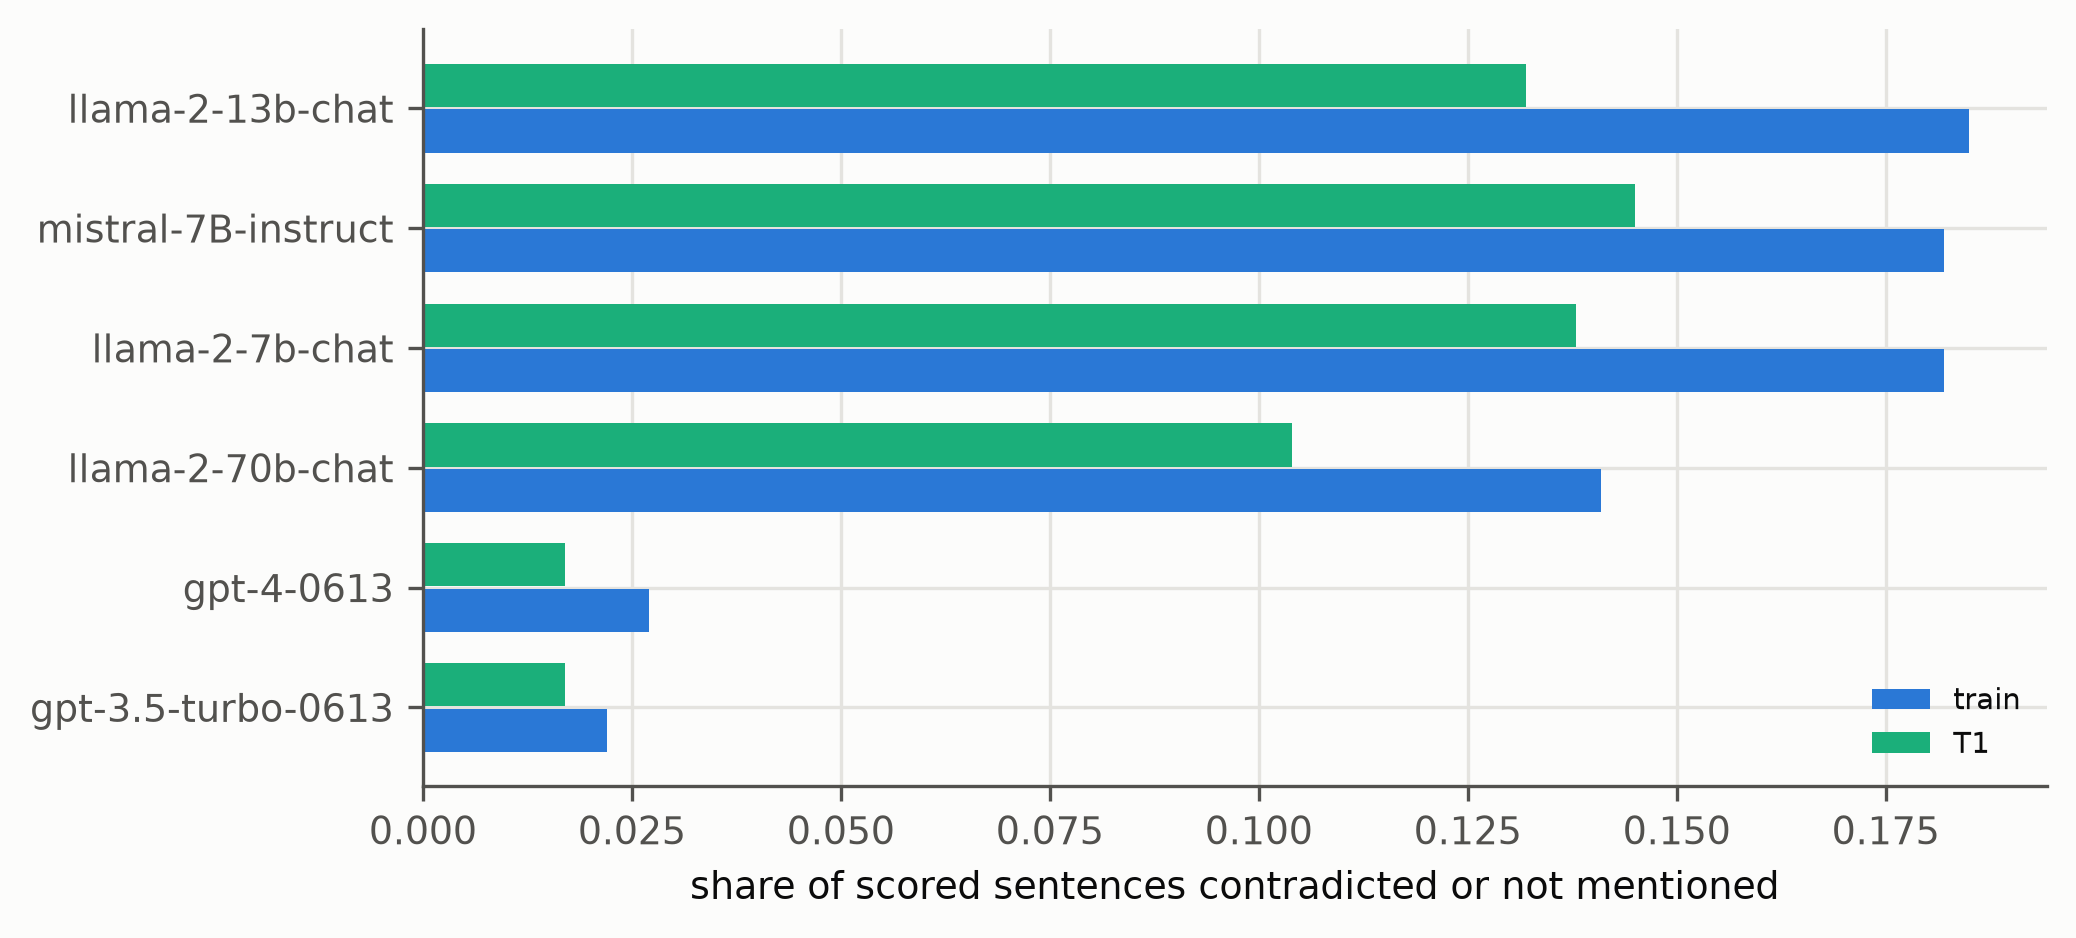
\includegraphics[width=0.9\textwidth]{images/eda/unsupported_by_generator.png}
\caption{Quota di frasi contraddette o non menzionate in base al modello che ha scritto la risposta, nel training set e
in T1.}
\label{fig:data-generators}
\end{figure}

\paragraph{Le risposte di test sono più pulite di quelle di addestramento.} In ogni task e per ogni generatore, la quota
di frasi contraddette e non menzionate è più bassa in T1 che nel training set. Nel question answering, per esempio, è
contraddetto lo 0.6\,\% delle frasi di T1, contro l'1.6\,\% di quelle del training set. Di conseguenza, le metriche che
dipendono dalla frequenza di base delle classi, come la precisione o l'F1 sulle classi minoritarie\footnote{La \emph{precisione} è la quota delle
predizioni di quella classe che risultano corrette, e per questo cambia con la frequenza della classe anche quando il
modello resta lo stesso. L'F1 è la media armonica delle due.}, non sono confrontabili tra dev set e test set, perché il dev set, estratto dal training set, ne conserva la distribuzione. Le metriche principali sono quindi la balanced accuracy, la recall per classe e l'AUROC, che dalla frequenza di base non dipendono.

\paragraph{Le contraddizioni sono per lo più evidenti.} Circa l'85\,\% delle frasi contraddette del training set deriva
da span annotati come conflitti \emph{evidenti}, per esempio numeri o nomi sbagliati, mentre soltanto 147 derivano da
conflitti \emph{sottili}. La classe contraddetta è quindi composta soprattutto da contraddizioni palesi, e le
contraddizioni sottili non possono essere valutate separatamente.

\paragraph{Esistono indizi superficiali, e definiscono le baseline.} Due indizi semplici predicono le etichette senza
verificare la frase rispetto al documento. Il primo è la sovrapposizione lessicale, cioè la quota delle parole di
contenuto della frase che compaiono anche nel documento; le parole di contenuto sono quelle che restano escludendo le
parole funzionali, come articoli, preposizioni e verbi ausiliari. In tutti e tre i test set questa quota è più alta per
le frasi supportate che per quelle contraddette e non menzionate (Figura~\ref{fig:data-overlap}). Usata da sola come
punteggio, separa le frasi supportate da quelle non supportate con un AUROC di 0.74 su T1 e di 0.70 su T3. Il secondo
indizio è la formulazione della frase. Nel data-to-text, un classificatore che vede soltanto la frase raggiunge una
balanced accuracy a tre classi di 0.66, perché nelle descrizioni di Yelp alcuni dettagli vengono inventati spesso, come
il numero di recensioni o la disponibilità di Wi-Fi o del parcheggio con valet. Nel question answering e nella
summarization, invece, lo stesso classificatore resta al livello del caso (0.36 e 0.35), e lo stesso accade su T3
(0.33), dove la costruzione contrastiva del dataset elimina l'indizio. Un verificatore è utile solo nella misura in cui
batte questi indizi, per cui entrambi sono riportati come baseline, task per task.

\begin{figure}[htbp]
\centering
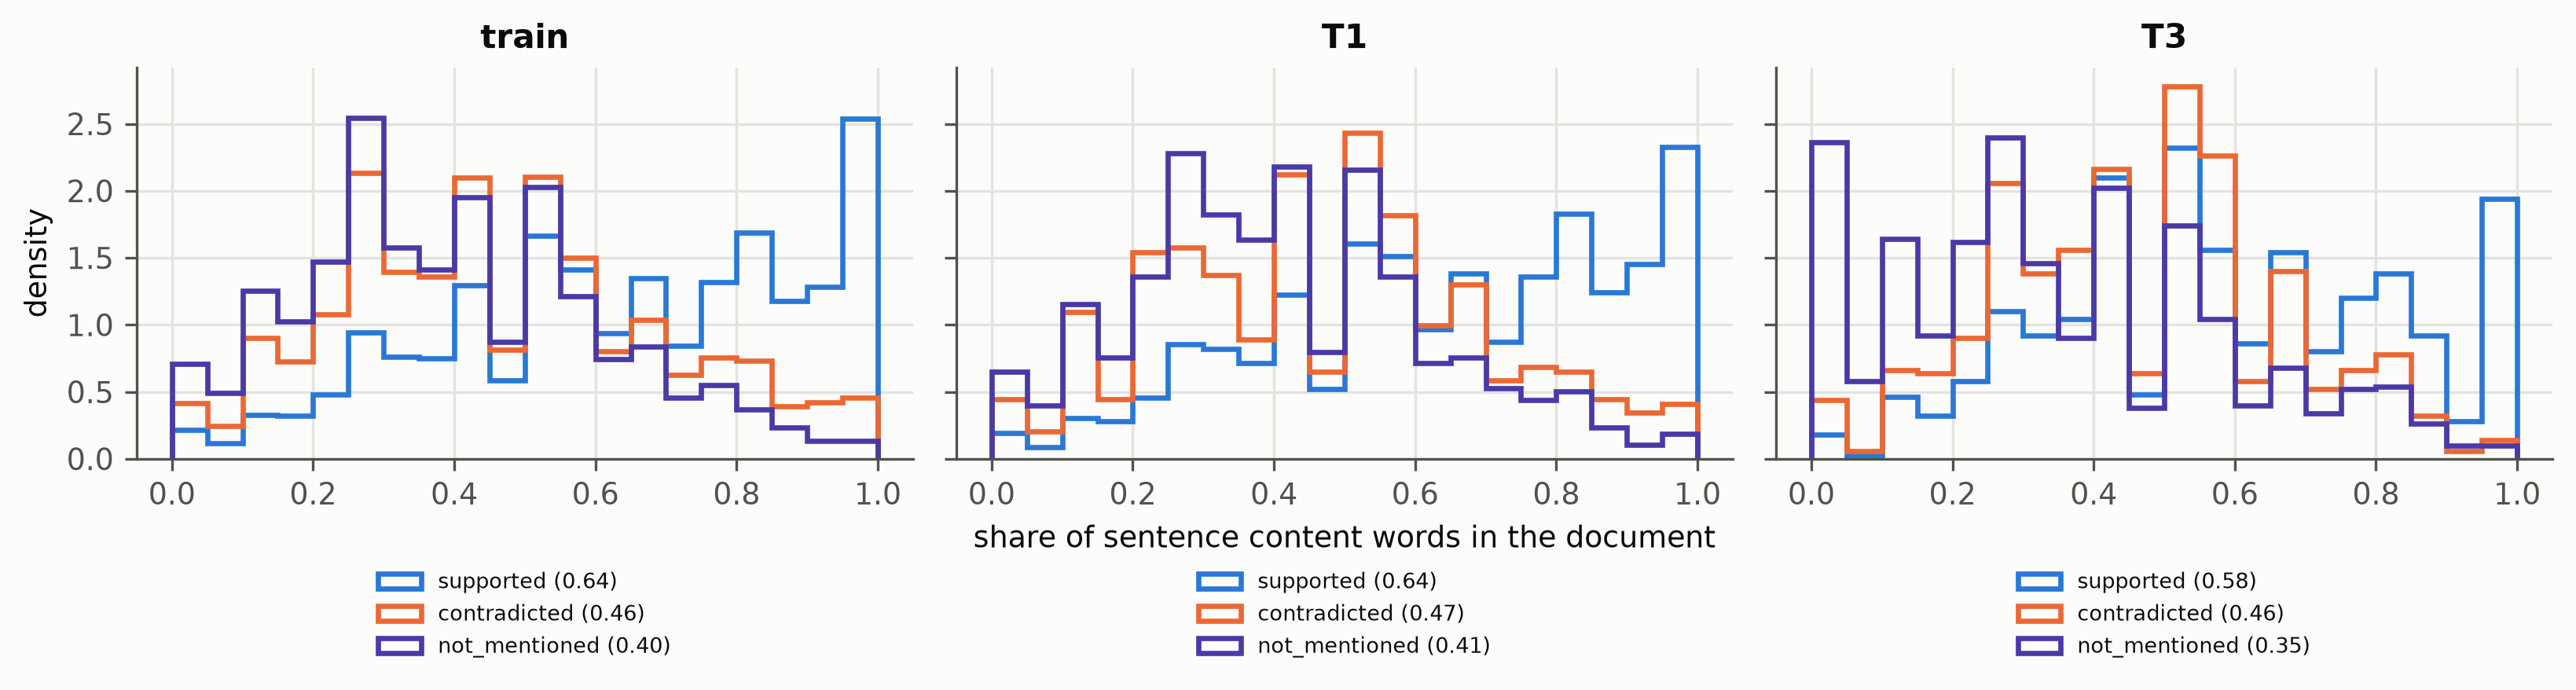
\includegraphics[width=\textwidth]{images/eda/overlap_by_class.png}
\caption{Sovrapposizione lessicale tra una frase e il suo documento, cioè quota delle parole di contenuto della frase
presenti nel documento, per classe, nel training set, in T1 e in T3. Tra parentesi è indicata la media.}
\label{fig:data-overlap}
\end{figure}

Infine, le frasi non supportate non si concentrano alla fine della risposta. La prima frase è raramente non supportata,
mentre la quota di frasi non supportate raggiunge il massimo tra la terza e la quinta posizione e resta tra l'8 e
l'11\,\% nelle posizioni successive (Figura~\ref{fig:data-position}). Anche le risposte lunghe, quindi, contengono errori
verso la fine, e l'accuratezza per valori elevati di $K$ resta rilevante.

\begin{figure}[htbp]
\centering
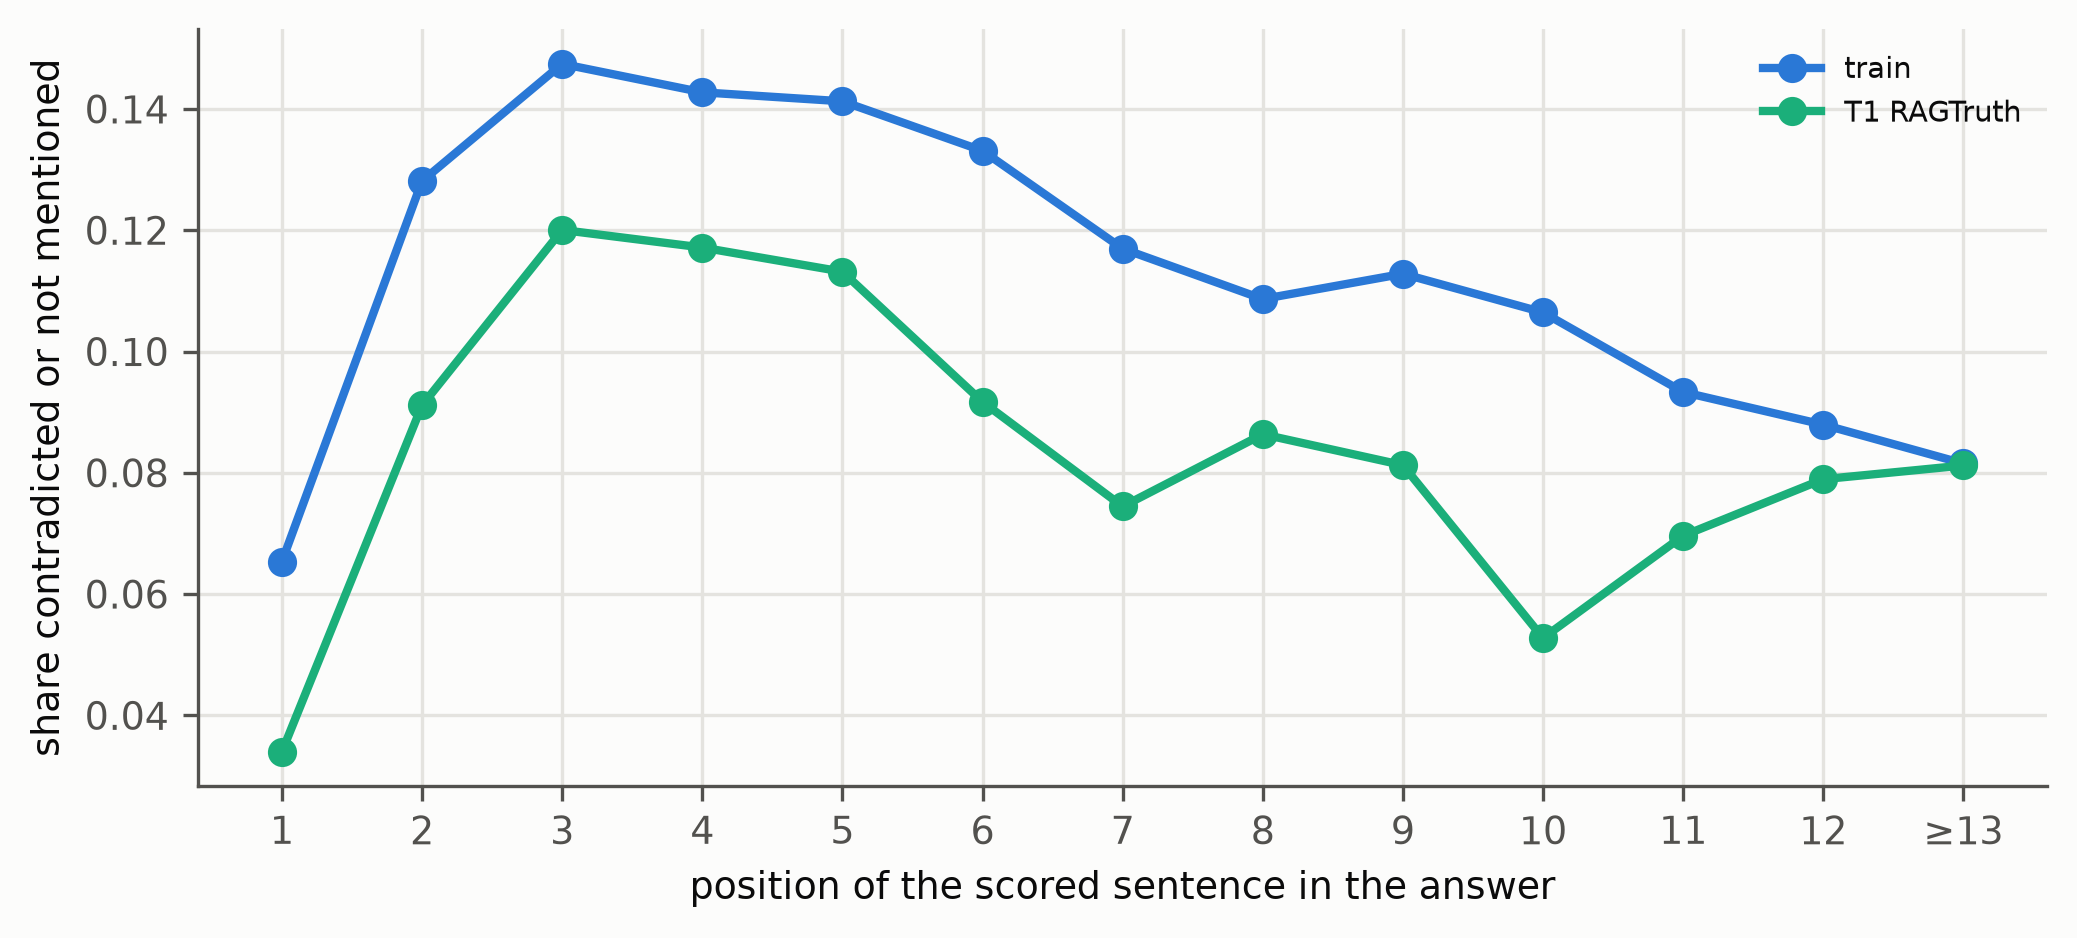
\includegraphics[width=0.9\textwidth]{images/dataset/unsupported_by_position.png}
\caption{Quota di frasi contraddette o non menzionate in base alla posizione della frase nella risposta.}
\label{fig:data-position}
\end{figure}

\section{Controllo del leakage}
\label{sec:data-leakage}

Il leakage, cioè la presenza tra i dati di addestramento di informazioni del test set, renderebbe ottimistiche tutte
le metriche dei capitoli successivi. In questo dataset il rischio è concreto: RAGTruth contiene, per ogni documento,
più risposte scritte da modelli diversi. Se queste risposte finissero in split diversi, il modello vedrebbe in
addestramento proprio il documento su cui viene poi valutato. Per questo gli split sono definiti per fonte e mai per
frase, così che tutte le risposte relative a una stessa fonte cadano nello stesso split. A ogni costruzione del dataset viene inoltre eseguito un controllo automatico, che fallisce in due casi:
quando una fonte, un documento o una coppia (documento, frase) del training set o del dev set compare in uno qualsiasi
dei test set, e quando dev set e training set condividono una fonte. Sul dataset finale il controllo non ha rilevato
alcuna sovrapposizione di questo tipo. Il controllo elenca anche, senza bloccare la costruzione, le frasi che compaiono
con le stesse parole sia nei dati di addestramento sia in quelli di test, ma riferite a documenti diversi. Sono 788, e
sono tutte frasi standard del data-to-text, come ``The business has a rating of 4.0 stars.'': il modello generatore le
ripete per attività commerciali diverse, quindi la loro presenza nei dati di addestramento non anticipa alcuna
etichetta di test, che dipende sempre dal documento a cui la frase si riferisce. Resta un aspetto che non è possibile verificare: se i dataset pubblici usati qui
facessero parte dei dati di pre-training di Qwen2.5. È un limite comune alla maggior parte dei lavori su benchmark
pubblici.
